\documentclass[11pt]{elsarticle}
\usepackage{geometry}                % See geometry.pdf to learn the layout options. There are lots.
\geometry{letterpaper}                   % ... or a4paper or a5paper or ... 
%\geometry{landscape}                % Activate for for rotated page geometry
%\usepackage[parfill]{parskip}    % Activate to begin paragraphs with an empty line rather than an indent
\usepackage{multirow}
\usepackage{graphicx}
\usepackage{amssymb}
\usepackage{epstopdf}
\usepackage{natbib}
\usepackage{wrapfig}
\DeclareGraphicsRule{.tif}{png}{.png}{`convert #1 `dirname #1`/`basename #1 .tif`.png}
\graphicspath{{figures/}}

\title{Reproducing ParConnect for SC16}
\author{Marek Baranowski, Braden Caywood, Hannah Eyre, Janaan Lake, \\Kevin Parker, Kincaid Savoie, Hari Sundar, Mary Hall}
\address{School of Computing, University of Utah, Salt Lake City, Utah, USA}
%\date{}                                           % Activate to display a given date or no date

\begin{document}
\begin{abstract}
This paper describes our SC16 Student Cluster Competition team's efforts to reproduce the results of
an SC15 paper for an application called ParConnect.  This application finds connected components in graphs, specifically for De Bruijn graphs used in metagenomic assembly. We performed experiments running this application on a Dell PowerEdge cluster with Nvidia P100 GPUs and an Intel Omni-Path interconnect. Our results demonstrated that we could reproduce some but not all of the performance claims in the
original publication.  We expect that small data set sizes and differences in our cluster configuration account for the variation
in results.
\end{abstract}
\maketitle

\section{Introduction}
The ability to reproduce scientific computing results is essential to advancing algorithms and optimizations suitable for high-performance
computing.  At the SC16 conference, a new component of the Student Cluster Competition required teams to reproduce the results from 
a prior conference by reading a paper and installing the associated software on their cluster.  The overall competition involves a team of 
six undergraduates designing a new cluster from state-of-the-art hardware and software, running a set of required applications
on the hardware, and providing written and oral descriptions of the results.

This paper presents the results of the reproducibility exercise from SC16, using results that were collected during the conference.  The 
selected paper describes a new, distributed algorithm for finding connected components in graphs, specifically for De Bruijn graphs for
metagenomic assembly, within an application called ParConnect~\cite{Flick:2015}. Metagenomic assembly refers to the study of microbial
genomes directly obtained from environmental samples, thus sampling the aggregate genomes of many different species.  In a de Bruijn 
graph, vertices are strings of size \textit{k}, and edges represent (\textit{k}-1)-long suffix-prefix overlaps between strings.

A bucketing algorithm based on tuples representing undirected edges is used to identify connected components in the graph. 
The application uses MPI to distribute edges across the hardware nodes in a cluster.  The number of edges considered is initially
distributed evenly across the MPI ranks. A sorting and reverse procedure allows the ranks to find nodes that are connected between MPI
ranks, by checking the last element after the sort. 
The authors describe two different implementations of their algorithm:
\begin{itemize}
\item \textit{Active Partition (AP):}
Tuples that are part of a
component that is not connected to any other nodes are removed. This allows the algorithm to focus on finding new components, while
ignoring tuples that are part of a connected component and thereby reducing workload. 
\item \textit{Active Partition with Load Balancing (AP\_LB):}
As a further enhancement, after each BFS iteration, the tuples are redistributed so that all ranks are load balanced. 
\end{itemize}

The authors claim that the active partition makes the distributed breadth-first search (BFS) connected-component algorithm faster.   By adding load balancing, the algorithm runs faster, as all ranks are working on the same amount of data. We are testing the authors' assertion that the na{\"i}ve approach is slower than the active partition approach and load balancing further enhances the active partition algorithm. In addition, we are testing the weak scaling behavior of the algorithms.

\section{Cluster and Software Details}
Our team partnered with Dell, Nvidia and Intel to build the cluster.  The resulting system
has two Dell PowerEdge C1430 nodes. Each node has two Intel Xeon E5-2640 v4 CPUs clocked at 2.40 GHz. Each socket has 64 GB of DDR4 memory clocked at 2133 MHz, with a total of 256 GB of memory across the entire cluster. For interconnect, we use four Intel Omni-Path Fabric 100 series cards. We have one Omni-Path card tied to each socket's PCIe 3 bus with 8 lanes; this gives a theoretical bandwidth of 7.88 GB/s per connection.  The cards are connected directly in a dual-plane configuration between the two nodes, forming a ring topology between the four sockets. The cluster runs CentOS 7 with Linux kernel version 3.10.0-327.36.3.el7.x86\_64.
 To compile ParConnect we clone the repository as indicated in the instructions. We use cmake to configure the build with
 -DBENCHMARK\_ENABLE\_CONN=ON for benchmarking purposes. We use Intel MPI because we found it works best with the Omni-Path interconnect.  We use GCC 4.9.2 and Intel MPI 5.1.3 Build 20160120. Prior the competition, we pre-compiled ParConnect with each of the three algorithms, Na{\"i}ve, AP and AP\_LB. 
 
 \section{Results}
 The data sets are described in Table~\ref{tab:datasets}. These data sets were provided by the competition organizers,
 and were chosen such that among all competitor's cluster nodes, the node with the least amount of memory could complete the experiment.
% First table
\begin{table}[htp]
\centering
\begin{tabular}{l|c|c|}
\cline{2-3}
                                           & \textbf{Edge Count} & \textbf{\begin{tabular}[c]{@{}c@{}}Connected \\ Components
                                           \end{tabular}}\\\hline
\multicolumn{1}{|l|}{\textbf{small.fastq}} & 90,665,399            & 1,929,553\\ \hline
\multicolumn{1}{|l|}{\textbf{large.fastq}} & 442,461,650           & 9,006,212\\ \hline
\end{tabular}
\caption{Edge counts and connected component counts for the two data sets.}\label{tab:datasets}
\end{table}

% Second table
\begin{figure}[htp]
\centering
\begin{tabular}{|l|l|l|l|}
\hline
\multirow{3}{*}{\rotatebox{90}{Time (sec)\hspace*{1in}}} & \multicolumn{3}{c|}{\begin{tabular}[c]{@{}l@{}}Computation and communication runtime along the iterations\end{tabular}} \\ \cline{2-4} 
    &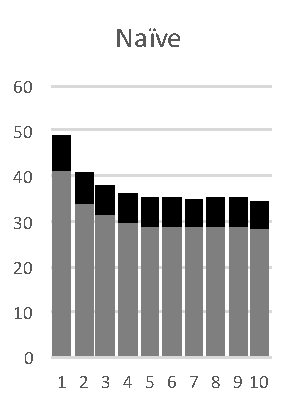
\includegraphics[width=.29\textwidth]{naivecompcomm}&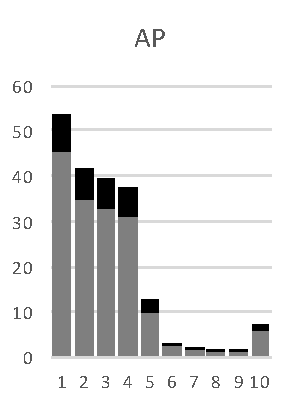
\includegraphics[width=.29\textwidth]{apcompcomm}&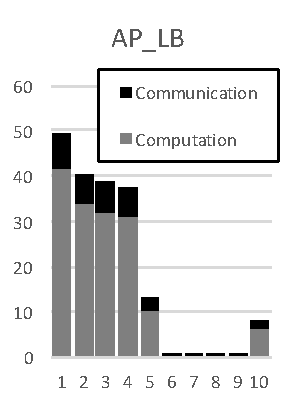
\includegraphics[width=.29\textwidth]{aplbcompcomm}\\ \cline{2-4} 
    & \multicolumn{3}{c|}{Iterations}\\ \hline
\end{tabular}
\caption{Time spent during communication and computation on \textbf{large.fastq} for each algorithm on 40 processes.}
\label{fig:compcomm}
\end{figure}

%Third table
\begin{figure}[htp]
\centering
\label{my-label}
\begin{tabular}{|l|l|}
\hline
Na{\"i}ve & 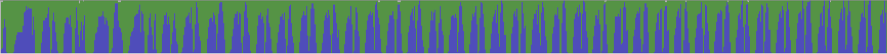
\includegraphics{naiveallinea} \\ \hline
AP & 
\includegraphics{apallinea} \\ \hline
AP\_LB & 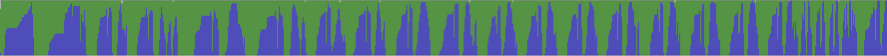
\includegraphics{aplballinea} \\ \hline
\end{tabular}
\caption{Performance timelines collected by Allinea Forge and displayed by the MAP tool. Compute time (green) and communication time (blue) is shown for each algorithm.}
\label{fig:allinea}
\end{figure}

Performance results are shown in Figure~\ref{fig:compcomm}; these times were reported by ParConnect's internal logging.
For computation time and communication time on large.fastq, we see results similar to those in Flick~\cite{Flick:2015}. The Na{\"i}ve algorithm is slowly falling as the number of iterations increases, and for AP and AP\_LB, we can see slight reductions in times in each iteration. The biggest drop off in times is most apparent in iterations 6-9, but overall AP\_LB uses less time per iteration. Comparing Allinea Forge results with the ParConnect's self-reported internal-timing, we see a big discrepancy in the percentage of time spent communicating versus computing. In particular, the timing information from ParConnect indicates that MPI takes up approximately 20\% of the time, however Forge indicates that 44\% of the time is in MPI calls. From Forge MAP's timeline (Figure~\ref{fig:allinea}), we can see pthread activity during some MPI portions of the execution. ParConnect's internal timing counts communication time and computation time separately. The discrepancy between ParConnect's self-reported times and Forge's measured times is likely due to internal timing being unaware of the behavior of the MPI runtime. Communication may begin between ranks before all ranks have completed their computation portion, or computation on some ranks begins before an entire collective communication has completed. If the MPI runtime behaved the way assumed by ParConnect, Figure~\ref{fig:allinea} should nearly be bands of green and blue. This would indicate the entire application is either in a communication state or a computation state at a given point in time.
%Fourth table
\begin{figure}[htp]
\centering
\begin{tabular}{|l|l|l|l|}
\hline
\multirow{3}{*}{\rotatebox{90}{Count of tuples (millions)\hspace*{.55in}}} & \multicolumn{3}{c|}{\begin{tabular}[c]{@{}l@{}}Balance of work across processors along the iterations\end{tabular}} \\ \cline{2-4} 
    &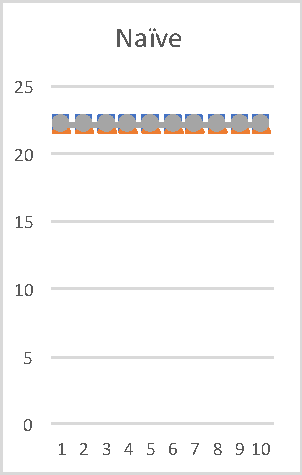
\includegraphics[width=.29\textwidth]{naivebalance}&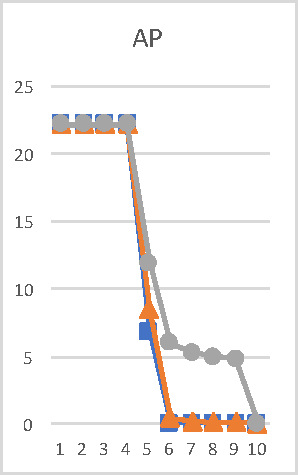
\includegraphics[width=.29\textwidth]{apbalance}&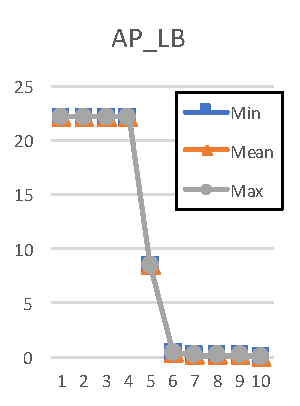
\includegraphics[width=.29\textwidth]{aplbbalance}\\ \cline{2-4} 
    & \multicolumn{3}{c|}{Iterations}\\ \hline
\end{tabular}
\caption{Min, mean and max tuple counts per iteration for each algorithm on 40 processes.}
\label{fig:loadbalance}
\end{figure}

For the active tuple count we see behavior consistent with that of the paper, as demonstrated in Figure~\ref{fig:loadbalance}. The na{\"i}ve algorithm maintains the same number of tuples throughout all BFS iterations. Active partition shows the number of tuples dropping at iteration 5. This is consistent with the algorithm finding connected components that have no out-going edges to other active tuples. Notably, we see an improvement in load balance beginning at iteration 5. The mean number of tuples in iteration 6-9 indicates most ranks have almost no tuples while there are a few ranks with about 5 million tuples. Finally, the AP\_LB algorithm shows that all processes maintain the same number of active tuples as indicated by the maximum and minimum. Specifically, the difference between the minimum number of tuples and maximum number of tuples is one throughout all iterations. This is consistent with the algorithm balancing the work between all ranks.
% Fifth table
\begin{figure}[htp]
\centering
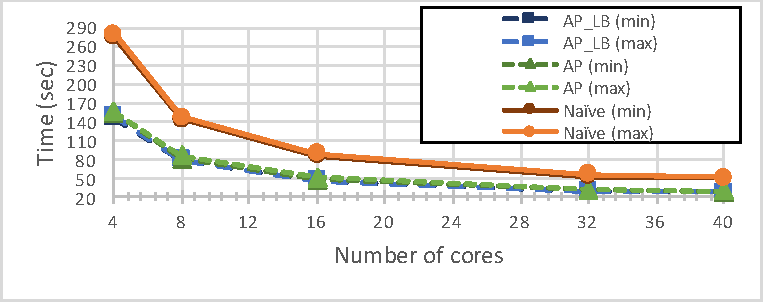
\includegraphics[width=.9\textwidth]{allruntimes}
\caption{Runtimes for \textbf{small.fastq} on 4, 8, 16, 32 and 40 processes.}
\label{fig:runtimes}
\end{figure}

\begin{figure}[htp]
\centering
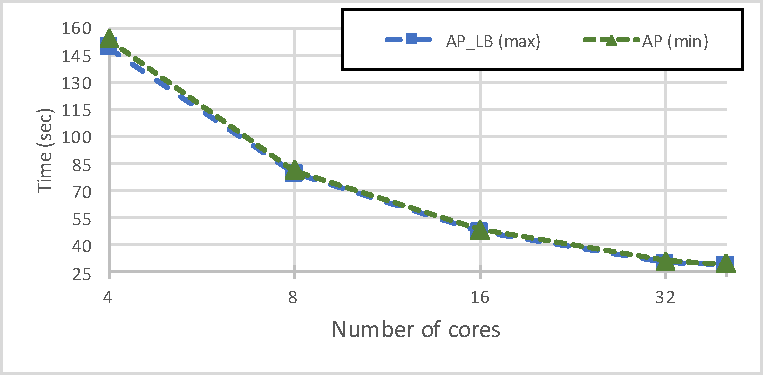
\includegraphics[width=.9\textwidth]{zoomedapaplb2}
\caption{Expanded AP and AP\_LB runtimes. Minimum and maximum times respectively.}
\label{fig:expruntimes}
\end{figure}
For the scaling study (Figure~\ref{fig:runtimes}), we can clearly see that the na{\"i}ve algorithm takes approximately twice as long as either AP or AP\_LB, consistent with the paper's claim that removing connected components speeds up the algorithm. A substantial divergence from the paper is apparent from this experiment; AP and AP\_LB perform nearly identically. While not visible in the graph, the maximum runtime for AP\_LB is always about two seconds faster than the minimum runtime of AP. Figure~\ref{fig:expruntimes} shows an expanded graph for the minimum and maximum run times of AP and AP\_LB respectively. This is not consistent with the paper's claim for load balancing improving performance: the graph suggests AP\_LB should be about 1.7 times faster than AP. We can see that the author's claim that AP\_LB is faster than AP, however, we see diminishing returns with increasing cores.


\section{Conclusion}
   Many of the claims in the paper were reproduced in this study. The active partition algorithm does reduce the number of work items per process as claimed in the paper. Figure 1 shows that this approach improves performance relative to the na{\"i}ve algorithm. Figure 3 shows that the algorithm balances the load of tuples between the processes as seen in the AP\_LB plot. We also see in the scaling study that the runtimes decrease as we move from the na{\"i}ve algorithm to the active partition algorithm, and another improvement when moving to the active partition with load balancing algorithm.
   In the scaling study, we did not witness a significant speed up when moving from AP to AP\_LB. This could be caused by a number of factors. It is possible the data set is too small to benefit from the load balancing approach, or the data set's components are constructed in such a way that load balancing does not help. Another possible cause is the specific configuration of our machine. We have two high bandwidth paths between each socket, requiring at most one hop across the Intel QuickPath Interconnect to get data to a socket on another node. Our machine is not like the machine used in the paper where there were a number of machines used and MPI communication latencies and bandwidth may be constrained. Our cluster could be concealing the cost of the MPI communication versus computation time. For 8 MPI ranks on iteration six, AP has min, mean, max tuples of 5410, 153231, 944395 respectively. For comparison, AP\_LB has 153231 active tuples on iteration 6 with 8 MPI ranks. The time to get from iteration 6 to iteration 7 is .4s and .08s respectively, consistent with the maximum tuple load in AP being approximately 5 times higher than the maximum load of AP\_LB. From iteration 7 the algorithm quickly ends, and this is likely why we are not seeing the promised speed up from load balancing.

\bibliographystyle{plainnat}
\bibliography{main}

\end{document}  
